\documentclass[10pt,a4paper]{article}
\usepackage[latin1]{inputenc}
\usepackage{amsmath}
\usepackage{amsfonts}
\usepackage{amssymb}
\usepackage{graphicx}
\usepackage[width=16.00cm, height=22.00cm]{geometry}


\usepackage{siunitx}

\usepackage[acronym,translate=false]{glossaries}
\usepackage[backend=biber,style=bwl-FU,maxbibnames=99]{biblatex}
\addbibresource{bibrefs.bib}

\usepackage{setspace}
%\singlespacing
%\onehalfspacing
\doublespacing
%\setstretch{1.1

%\title{The Importance of Eddy-Topographic Interactions for Arctic
%	Ocean Dynamics and Steps Towards Improving Climate Models}
%\author{Mark Edward Forshaw\\ Department of Physics\\
%University of Oxford\\ E-mail: \url{forshaw@atm.ox.ac.uk}}


\newacronym{amoc}{AMOC}{Antarctic Meridional Overturning Circulation}
\newacronym{bas}{BAS}{British Antarctic Survey}
\newacronym{arp}{ARP}{Arctic Research Program}
\newacronym{ipy}{IPY}{International Polar Year}
\newacronym{awl}{AWL}{Atlantic Water Layer}
\newacronym{aomip}{AOMIP}{Arctic Ocean Model Inter-comparison Project}
\newacronym{pv}{PV}{potential vorticity}
\newacronym{gcm}{GCM}{Global Climate Model}
\newacronym{bso}{BSO}{Barents Sea Opening}

\nocite{cushman2011introduction}
\nocite{vallis2006atmospheric}

\title{Thesis}


\begin{document}

\maketitle


\section{Introduction}

\subsection{Arctic Ocean}


Despite its small size (only $3\%$ of the Earth's surface), the Arctic
Ocean is an important part of the global ocean and has the potential
to affect the world's climate in major ways. Located above
$70\,^{\circ}{\rm N}$, the Arctic is characterised by its seasonally
varying ice cap. This ice cap, along with its counterpart at the South
Pole, is a major contribution to the planet's albedo as well as being
a large reservoir for freshwater. The Arctic Ocean is a key component
in how the polar ice cap interacts with the climate and, in turn, how
the climate affects the ice cap. 
The Ocean itself is a highly stable body of water with strong stratification, 
which means that the water column can be divided into advective water masses.
The Arctic Ocean is commonly divided into four different layers (Figure \ref{fig:amap}):
The Polar Mixed Layer, which is a well mixed layer in
contact with the atmosphere and surface ice; the halocline, which acts as
reservoir of fresh water and penetrates to around ${\sim}200\,{\rm m}$; the \gls{awl},
which is body of warm salty water which originates from the North Atlantic and Nordic 
Sea via Fram Strait and typically sits at around ${\sim}400\,{\rm m}$ deep; and finally, 
the Polar Deep Water, defined by the water masses that aren't
able to communicate freely with the global ocean due to being trapped by the Arctic basin walls.



\begin{figure}
	\centering
	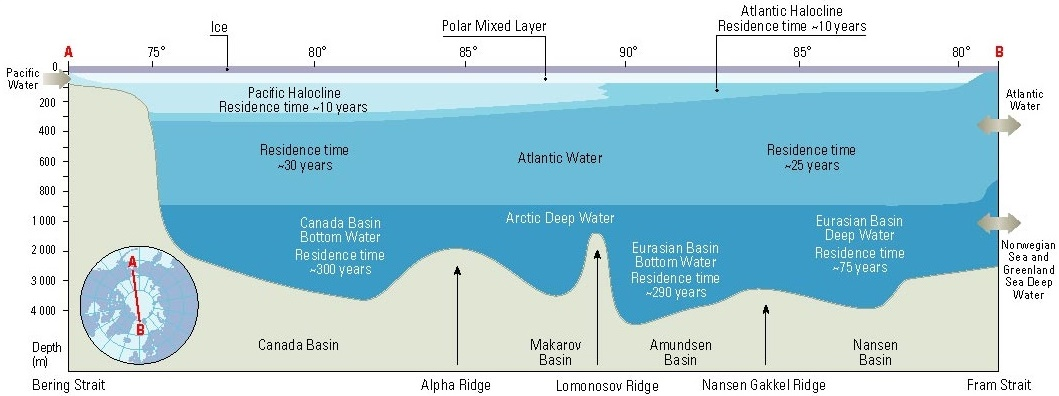
\includegraphics[width=\linewidth]{amap}
	\caption[\cite{wilson1998amap}]{  A schematic representation of the four-layer structure of the Arctic Ocean, with the Mixed Layer and Halocline
		above the Atlantic Water and Arctic Deep Water (\cite{aagaard1989role}). 
		The residence time for the different water masses are also shown (\cite{bonisch1995deep}). \cite{wilson1998amap}.}
	\label{fig:amap}
\end{figure}

\begin{figure}
	\centering
	\includegraphics[width=\linewidth]{Proshutinsky2005Circulation}
	\caption[\cite{proshutinsky2005arctic}]{ Two freshwater layer regimes (light 
		blue arrows) overlaying the cyclonic rim currents of the \gls{awl} (red arrows).
		Whilst the Freshwater regimes are vastly different from each other, the
		\gls{awl} is unaffected and remains persistently cyclonic.
		Topography is represented in the background running from 
		shallow water (light blue) to deep water (dark blue).  \cite{proshutinsky2005arctic}.}
	\label{fig:Proshutinsky2005Circulation}
\end{figure}

Because of the strong stratification, the forcing from the ocean surface 
struggles to penetrate deep into the ocean; and so whether forced directly by wind 
or by sea ice stress, the circulation
directly forced from the surface is contained within the Polar Mixed Layer 
and halocline in the upper ${\sim}200\,{\rm m}$ of the Arctic Ocean. 
This surface circulation has been well documented by observations
from cruises and moorings  dropped  from  the  ice  shelf  or  deployed  on 
the  shallower  continental  shelves (\cite{gerdes1997large}, \cite{jones2001circulation}). On the other hand, it's a very different
story for the circulation in the \gls{awl} and lower layers (Figure \ref{fig:Proshutinsky2005Circulation}). Observations made
inside the Ocean Basins rarely are able to profile the structure  and
circulation  below 500m  although much progress has been made here in the
past decade. This lack of observations means that  we  still only have  a  sense  of  the circulation 
of the \gls{awl} and the Deep  Waters.  The  observations  we  do 
have  infer stable cyclonic  rim  currents about each of the basins in the
\gls{awl} and it's believed that this trend extends through the Deep Water to the 
ocean floor.  Because of the highly stratified nature of the halocline, the surface forcing 
is likely to have little effect on the deeper ocean, which leaves the other 
two possibilities as the determining features.


\begin{figure}
	\centering
	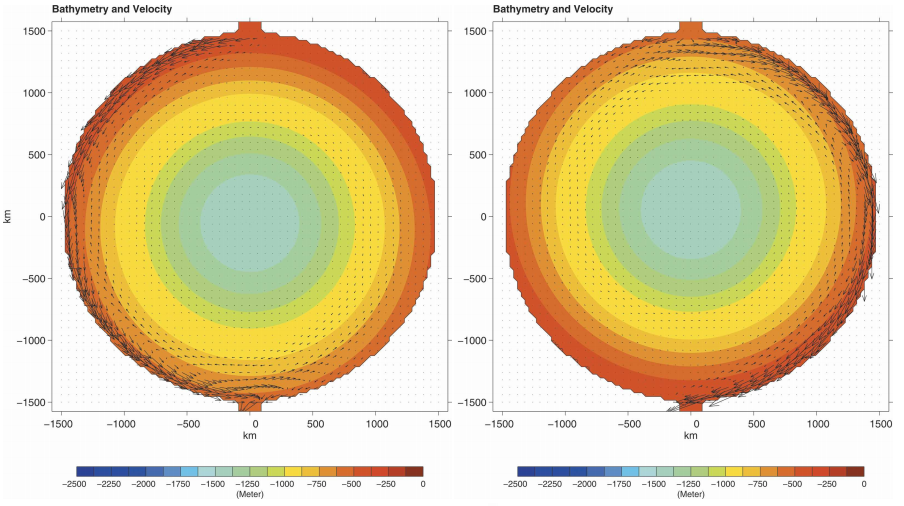
\includegraphics[width=\linewidth]{Yang2005}
	\caption[\cite{yang2005arctic}]{ The circulation of two simple barotropic
		models. The background colour is the model bathymetry. The left plot has
		a net influx of \gls{pv} (the inflow is shallower than the outflow) 
		and a cyclonic circulation whilst the right plot has net outflux of  \gls{pv} 
		and an anti-cyclonic circulation. \cite{yang2005arctic}.}
	\label{fig:Yang2005}
\end{figure}


\begin{figure}
	\centering
	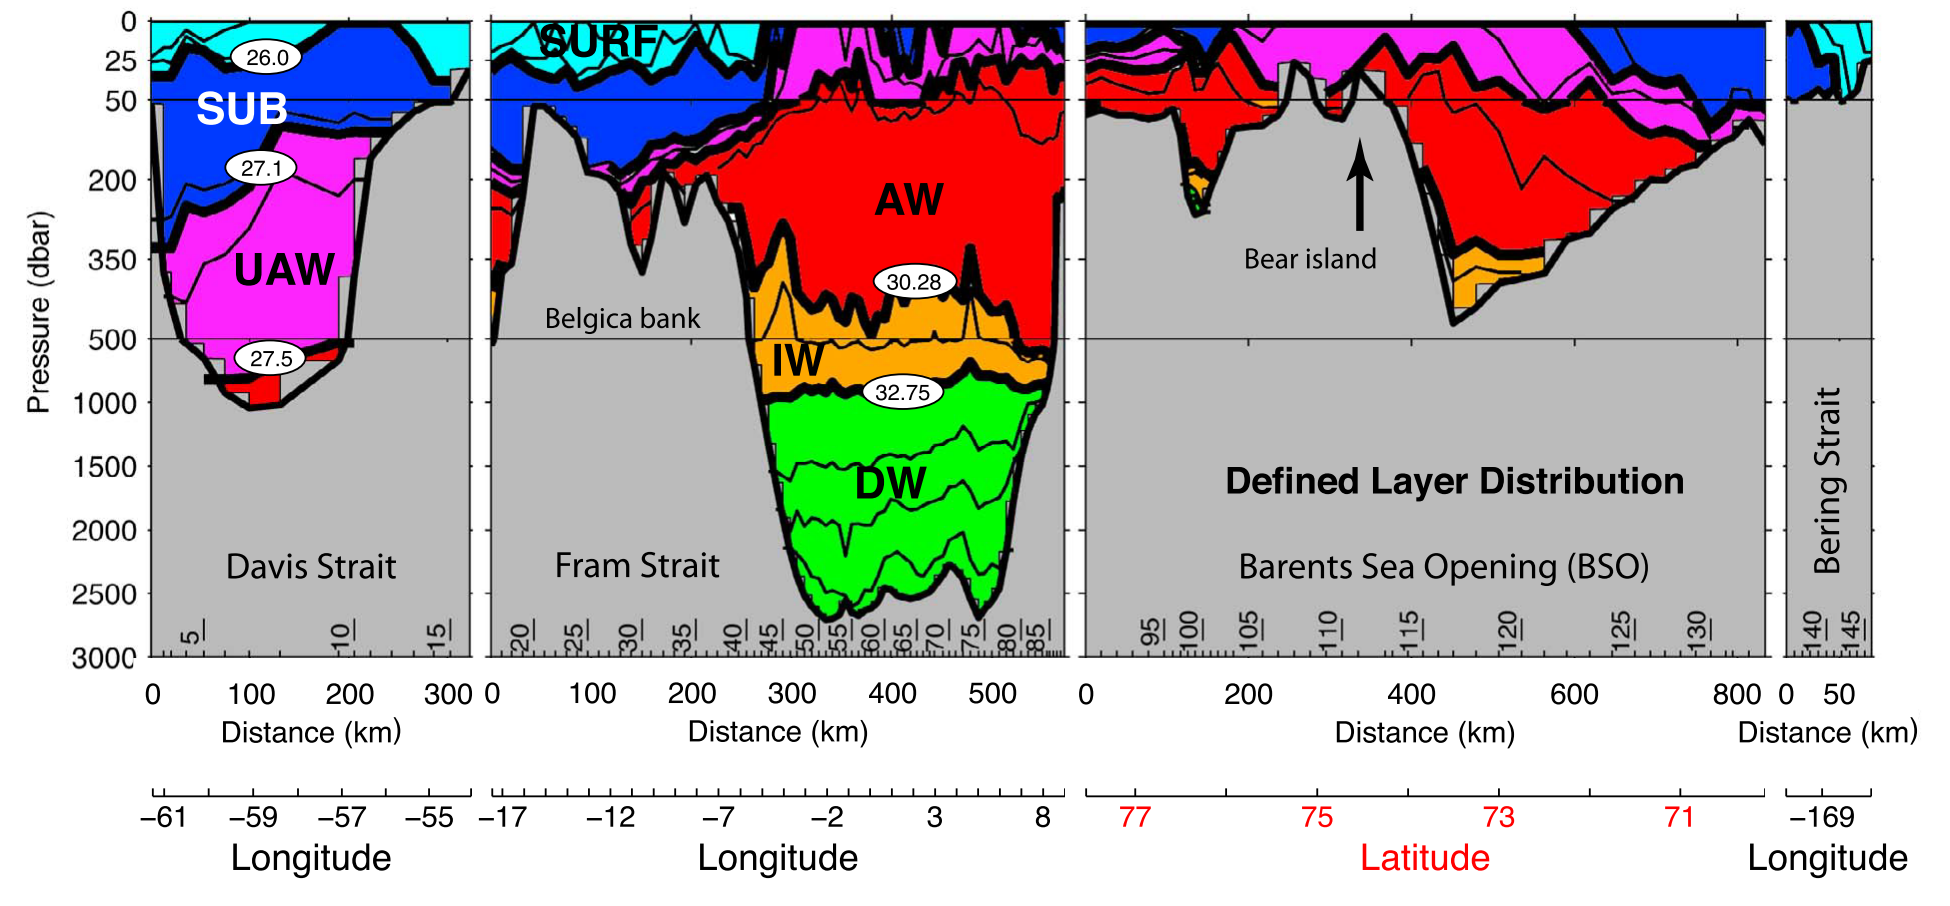
\includegraphics[width=\linewidth]{Tsubouchi2012Gateways}
	\caption[Adapted from \cite{tsubouchi2012arctic}]{The distribution of water masses and
		layer boundaries along sections of Davis Strait, Fram Strait, the \gls{bso} and
		Bering Strait. Water masses are labelled as SURF, the Mixed Layer; SUB, the halocline;
		UAW, AW, the upper and middle \glspl{awl}; and IW and DW, the intermediate and deep
		waters.  Adapted from \cite{tsubouchi2012arctic}.}
	\label{fig:Tsubouchi2012Gateways}
\end{figure}

\begin{figure}
	\centering
	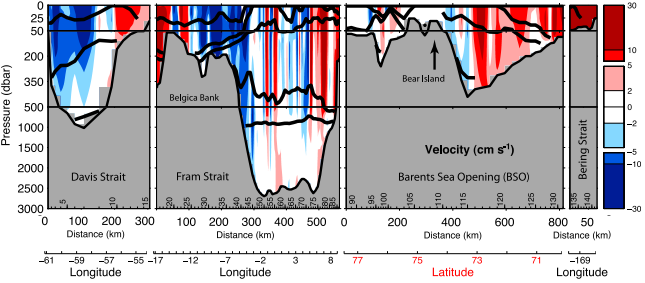
\includegraphics[width=\linewidth]{Tsubouchi2012Transport}
	\caption[Adapted from \cite{tsubouchi2012arctic}]{Velocity
		sections (${\rm cm} \, {\rm s}^{-1}$); bold black lines show defined water mass boundaries, and red (blue) colors show inflow
		to (outflow from) the Arctic.  Adapted from \cite{tsubouchi2012arctic}.}
	\label{fig:Tsubouchi2012Transport}
\end{figure}

There has been much discussion
into how the fluxes in and out of the Arctic could influence the circulation,
for example, by a forcing a balance of \gls{pv} within the region by
the fluxes of \gls{pv} though the boundaries. \cite{yang2005arctic} demonstrated how,
in an idealised barotropic model of a basin, controlling the flux 
of \gls{pv} through inflows and outflows
at the boundary, the circulation in the basin could be switched between cyclonic and
anti-cyclonic circulations (Figure \ref{fig:Yang2005}). This principle suggests
that the persistent cyclonic nature of the \gls{awl} implies that there is a 
net influx of \gls{pv} via the Arctic Gateways. Fortunately, permanent moorings 
covering the majority of the ocean gateways into the Arctic Ocean (Figure
\ref{fig:Tsubouchi2012Gateways}) have built
up a detailed picture of the transport in and out of the Arctic Ocean 
(\cite{tsubouchi2012arctic}, Figure \ref{fig:Tsubouchi2012Transport}). The net flux of \gls{pv} is then estimated by summing the distribution of \gls{pv}; given by $ \Pi_{i} = fQ_{i}/H_{i}$,
where $Q_{i}$ is the volume transport and $H_i$ the depth, for location $i$. 
Whilst there is a tendency for total to infer a positive influx of \gls{pv}, the
results are not convincing; \cite{munchow2006observational} shows that by including the
Canadian Archipelago in the \cite{yang2005arctic} calculation the flux can be negated whilst
\cite{tsubouchi2012arctic} demonstrates large variations of transport from the mean over time.
These factors make it unconvincing that its the \gls{pv} transport that determines the 
cyclonic nature of the \gls{awl}.
Hence, the deep water circulation in the Arctic Ocean is more likely determined by 
internal processes, which are poor understood in an Ocean with such sparse observations.


\begin{figure}
	\centering
	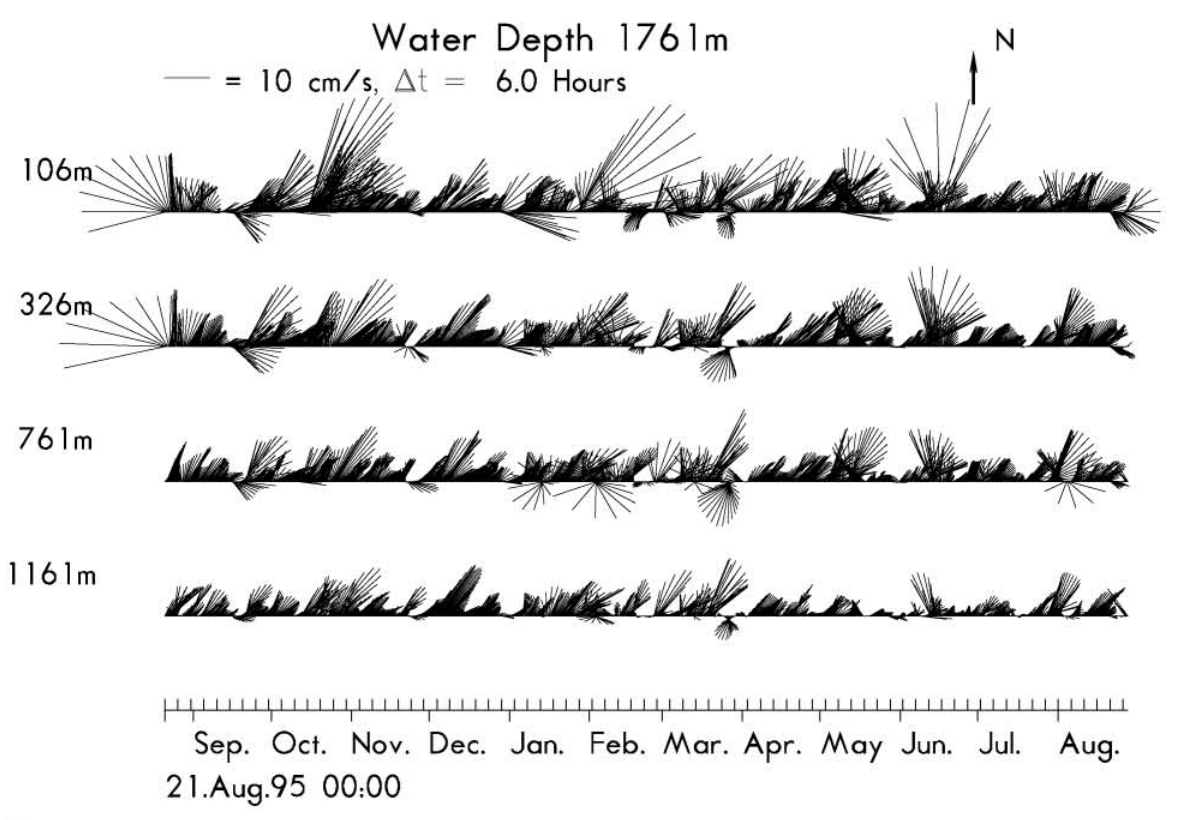
\includegraphics[width=\linewidth]{Woodgate2001Mooring}
	\caption[Adapted from \cite{woodgate2001arctic}]{A Velocity Stickplot 
		from a year-long mooring at \ang{78;30.8;} N, \ang{133;57.7;} E, west of the Lomonosov Ridge.  Adapted from \cite{woodgate2001arctic}.}
	\label{fig:Woodgate2001Mooring}
\end{figure}

A likely candidate for generating a cyclonic circulation in the Northern hemisphere is
geostrophic turbulence. A number of studies have demonstrated how, in an eddying system, 
sloping topography can generate along-topography flows (\cite{treguier1989topographically}, \cite{adcock2000interactions}, \cite{nost2008asymmetry}). Hence, in the absence of stronger
forcing, this effect is likely to become the dominant feature. The obvious question that then
comes to mind is how turbulent is the Arctic Ocean? Over recent years a large amount  of 
effort has been made to observe and catalogue eddies in the Arctic
(\cite{zhao2014characterizing}) and has demonstrated their prevalence in the Arctic Ocean.
Whilst these studies have frequently been focused on the halocline and the surface dynamics
there is good reason to believe that eddies also penetrate deep into the Arctic 
(Figure \ref{fig:Woodgate2001Mooring}, \cite{woodgate2001arctic}).

\subsection{Mean-Eddy Interaction Theory}

 Obviously, whilst observations play a vital role in understanding the Arctic
 Ocean and its role in the global ocean, it is limited by the sparsely available
 observations that only usefully reach back a handful of decades into the past.
 To be able to test possible scenarios and make future predictions it is vital
 that we have reliable simulations of the Arctic Ocean (\cite{proshutinsky2008toward});
 however, due to limitations
 in modern computing power and poor understanding of the unresolved processes 
 in the ocean this is, more often than not, far from reality.
 By attempting  to understand the physics behind these unresolved processes 
 and developing parameterisations that mimic their effect on the resolved ocean
 the value of computational models can be improved without dramatically increasing the
 computing power required.  Due to these computational limits a practical \gls{gcm} is 
 limited to a  resolution of the order of tens of kilometres. This means that with a 
 resolution  cut off at around $10 \textendash 100 \, \rm km$, 
 \glspl{gcm} are unable to fully resolve a large portion of the mesoscale turbulence that is
 observed in the physical ocean.
 
 The turbulent, chaotic nature of the ocean is caused by the non-linearity of its 
 governing equations. Because of this,  the discretisation of the equations generates cross-correlation, or eddy, terms when applying the 
 averaging operator,
 \begin{equation}
 \overline{\phi\psi} = \overline{\phi}\,\overline{\psi} + 
 \overline{\phi^{\prime}\psi^{\prime}},
 \label{non-lin average}
 \end{equation}
 where the prime denotes the residual, ${\phi^{\prime} = \phi - \overline{\phi}}$,
 and the ${\overline{\phi}}$ is the average of the variable ${\phi}$, used in
 the discretisation and satisfying
 the expected properties of an averaging operator.
 The discretised system has no knowledge of the residual terms and hence
 the contributions to the full system by these eddy terms are
 ignored in the discretised system. It is, therefore, this ``sub-grid scale process"
 that is missing from the model dynamics and so it is common practise to try and
 `close' the system by including a parameterisation of the eddy
 term in place of the term itself, which is usually dependent on the averaged 
 variables and some physical assumptions.
 
 The earliest ocean models (\cite{bryan1969numerical}) had vertical $z$-coordinate, or depth-coordinates, with simple horizontal and vertical Laplacian diffusion to act as 
 the closure. Whether these term are interpreted as a parameterisation for the effects
 of unresolved turbulence or simply as a numerical tool to avoid numerical noise at 
 the grid scale, the viscosity parameter is tuned such that the turbulent energy cascade is 
 dissipated at the grid scale whilst still allowing as active dynamics as possible. 
 Assuming modern day computing power this implies a horizontal viscosity of around 
 $10^{5} - 10^{7} \rm Pa \cdot s$, a viscosity more suited to peanut butter than 
 a saline ocean. A second problem with having such a strong horizontal diffusion is
 that it effectively large horizontal diffusion, or mixing of tracers when applied as
 an eddy parameterisation for tracer mixing. It has long been understood that tracers 
 mix much more along isopycnal surfaces than across them (\cite{iselin1939influence}, \cite{montgomery1940present}), which is a property which allowed for the definition of
 distinct water masses in the global ocean. Hence, by along excessive horizontal diffusion
 of tracers ocean models would be able to break up water masses much quick than
 is observed in the physical ocean. Hence, a more physically appropriate eddy parameterisation 
 was needed.
 
 And so, in today's world it seems obvious, parameterise eddies in such a way that their effect
 acts along isopycnal surfaces. The effort to do this in the 80's and early 90's gave birth
 to what is known as the Gent and McWilliams Parameterisation, first introduced in \cite{gent1990}.


\end{document}